\documentclass{jsarticle}
\usepackage{amsmath}
\usepackage{bm}
\usepackage{overcite}
\usepackage{wrapfig}
\usepackage{pifont}
\usepackage{fancybox}
\usepackage[dvipdfmx]{graphicx}
\renewcommand\citeform[1]{[#1]}
\newcommand{\FRAC}[2]{\leavevmode\kern.1em
 \raise.5ex\hbox{\the\scriptfont0 #1}\kern-.1em
 /\kern-.15em\lower.25ex\hbox{\the\scriptfont0 #2}}

\begin{document}

\begin{flushright}
B4 菊地

2014.5.27 
\end{flushright}

\begin{center}
\LARGE 高分子の分子運動

\large 〜輪読:エッセンシャル高分子 pp.107-114〜 
\end{center}
\section{並進運動}
\subsection{(6.69),(6.70)式を導出する}
高分子の運動は,並進運動,回転運動,内部運動の3つに分けて考えることができる.どの運動についても目標は,運動の速さと高分子の大きさなどの要素との関係を考えることである.運動の速さの指標としては「拡散定数」もしくは「緩和時間」を使っている.

まずひっかかるのが,(6.69)式と(6.70)式である.(6.69)式は教科書通りにやれば確かにそうなるが,なにかしっくりこない.もっとイメージしやすい方法で考えてみたい.実際に高分子のランダムな動きというものを考えてみることにしよう.

溶液中のランダムコイル状高分子は,複雑な運動をしている.まずは細かい運動は無視して並進運動,つまり高分子の重心の動きだけを考えてみよう.溶液中を粒子が動くイメージである.ランダムな動きをするものを追跡するときには,物理量の変動を特徴づけるために,異なる時刻における物理量の相関を考えることがある.平均を定義しやすい物理量の場合は,2つ目の運動である回転運動のところで出てくる時間相関関数というものを考えるのが普通である.しかし,分子の重心位置は平均が定義しにくい(ランダムに動く粒子がいる場所の平均,というものは考えにくい).そこで,このような場合は,物理量$X$について,$t$だけ時間が経ったときの変化の2乗平均
\begin{equation}
\langle (X(t)-X(0))^2 \rangle
\end{equation}
を考えると便利である~\cite{土井}.教科書では重心の位置ベクトル$\bm{R}_{\scalebox{0.5}{G}}$を使って書いているが,まずは(1)式の物理量$X$を一次元における粒子の位置として議論していく.溶液中の高分子の運動はブラウン運動とみなすことができるので,酔歩を考えていくのがよい\footnote{酔歩の連続モデルは拡散過程と等価である~\cite{米沢}.}.そして連続的に動かすためには,移動の幅を無限小にすればよい.$\varDelta t$という時間の間に,$\varDelta x(>0)$だけ右に動く確率が0.5,左に動く確率が0.5だとすると,ある時刻$t+\varDelta t$に粒子が位置$x$に来る確率は,
\begin{equation}
p(x,t+\varDelta t)=\dfrac{1}{2}p(x-\varDelta x,t)+\dfrac{1}{2}p(x+\varDelta x,t)
\end{equation}
と表せる.普通の一次元酔歩である.左辺について1次まで,右辺について2次までテーラー展開してから$\varDelta t$で割ると,
\begin{equation}
\frac{\partial p(x,t)}{\partial t}=\frac{(\varDelta x)^2}{2\varDelta t}\frac{\partial p^2 (x,t)}{\partial x^2}
\end{equation}
となる.この式はひとまず置いておこう.

さて,時間$t$で$X(t)$まで移動したとすると,それは$\varDelta t$で$\varDelta x$移動するという事柄が$t/\varDelta t$回起きたということである.各$\varDelta x$は$\varDelta X_i(=X(t_i)-X(t_{i-1}))$であり,それらはランダムであるから,
\begin{equation}
\langle \varDelta X_i \rangle=0
\end{equation}
となるのは明らかである.しかし,二乗平均はゼロにはならず,
\begin{equation}
\langle (\varDelta X_i)^{2} \rangle = (\varDelta x)^{2}
\end{equation}
である.同じようにして,$\langle (X(t)-X(0) \rangle$はゼロになるが,二乗平均はやはりゼロにはならない.各$\varDelta t$での二乗平均が(5)式で表され,それが$t/\varDelta t$回起きるのだから,
\begin{equation}
\langle (X(t)-X(0))^2 \rangle =\dfrac{t}{\varDelta t} (\varDelta x)^2
=\dfrac{(\varDelta x)^2}{2 \varDelta t} 2t
\end{equation}
である.(3)式に合わせるために変形してある.

連続モデルにするには,$\varDelta t \to 0$ , $\varDelta x \to 0$にするのだが,移動が起きるためには$\dfrac{(\varDelta x)^2}{2 \varDelta t}$が有限値でなくてはならない. なのでその有限値を$D_0$とおいておこう.
\begin{equation}
D_0 \equiv \dfrac{(\varDelta x)^2}{2 \varDelta t}
\end{equation}
そうすると,(6)式は
\begin{equation}
\langle (X(t)-X(0))^2 \rangle = 2D_0 t
\end{equation}
となる~\cite{米沢}.これは一次元で考えた場合なので,教科書にあるような三次元モデルにしたいならば,以上のようなことが$y$方向,$z$方向にも起きていると考えて,移動の二乗平均が3倍であるとすればよい(?)~\cite{戸田}  \footnote{始めの酔歩のところを三次元にして計算しなおすのがよいかもしれない.一つの動きが起きる確率が\FRAC{1}{2}だったのが\FRAC{1}{6}になるのだから,ここの係数が6になる??.ちょっとわからん.}.
\begin{equation}
\phi (t) = 3 \langle (X(t)-X(0))^2 \rangle = 6 D_0 t
\end{equation}
ただし,教科書では$D_{\scalebox{0.5}{G}}$としている.これが(6.69)式である.

さて,ほうっておいた(2)式は
\begin{equation}
\frac{\partial p(x,t)}{\partial t}=D_{\scalebox{0.5}{G}} \frac{\partial p^2 (x,t)}{\partial x^2}
\end{equation}
となる.$p(x,t)$は三次元で考えれば,濃度としてしまってよいだろう.このようにして,上で導出した$D_{\scalebox{0.5}{G}}$を使って拡散方程式も書けることが分かった.$D_{\scalebox{0.5}{G}}$はどちらの式でも,溶液中の高分子の拡散の速さを決めている.これで(6.69),(6.70)式が導出できた.



\subsection{(6.71),(6.73)式を導出する}
前節で,移動の二乗平均と拡散方程式では同じ定数$D_{\scalebox{0.5}{G}}$が出てきて,その定数は拡散のスピードを決めていることが分かった.実際には,拡散のスピードは高分子の形や溶媒の粘度などで決まりそうな気がする.次は,この定数が高分子のほかの要素(大きさ,形.結局は高分子を剛体球とみなしてその半径で表せることになる)でどのように記述できるかを考えていく.まず,Einsteinの関係式を導出する前に,(6.71)式と(6.73)式について考える.

この二つの式が主張するのは,高分子が外力に比例した速度で動き,その比例係数がしかじかと書けるということである.いやいや,力学によれば,外力がかかれば加速度が生じるのではなかったか?まずはこの現象について考えよう.

現実の系では,移動する物体には抵抗力が生じることが多い.空気抵抗や摩擦がそれである.この抵抗力は,移動の速さ$v$の効き方によって慣性抵抗と粘性抵抗に分けられる.これを無視してしまえば,先ほど述べたように加速度が生じるのであるが,高分子の溶液中での移動ではこの抵抗力は無視できない.ニュートンによれば,慣性抵抗$f_I$は次式で与えられる(以下の議論は球状物体についてである).
\begin{equation}
f_I = \frac{1}{4} \pi \rho _0 r^2 v^2
\end{equation}
$\rho _0$は流体の密度,$r$は球状物体の半径である\footnote{これは速さ$v$があまり大きくない場合について成り立つ式である.より速く移動する場合は,\FRAC{1}{4}をもう少し大きくしなければならないようである.これについては文献[9]が詳しい.実際に実験と比較して議論している.}.

一方,粘性抵抗は次式で与えられる\footnote{文献[4]が詳しい.}.
\begin{equation}
f_v = 6\pi \eta rv
\end{equation}
$\eta$は流体の粘度係数である.これをストークスの法則という.この式において$\zeta=6\pi \eta r$とすれば,教科書の(6.71)式のように書けてしまう.つまりどういうことだろうか.教科書では慣性抵抗を無視して粘性抵抗だけを考えているのである.では,なぜ慣性抵抗を無視できるのだろうか.
\begin{wrapfigure}{l}{20zw}
  \vspace*{-\intextsep}
  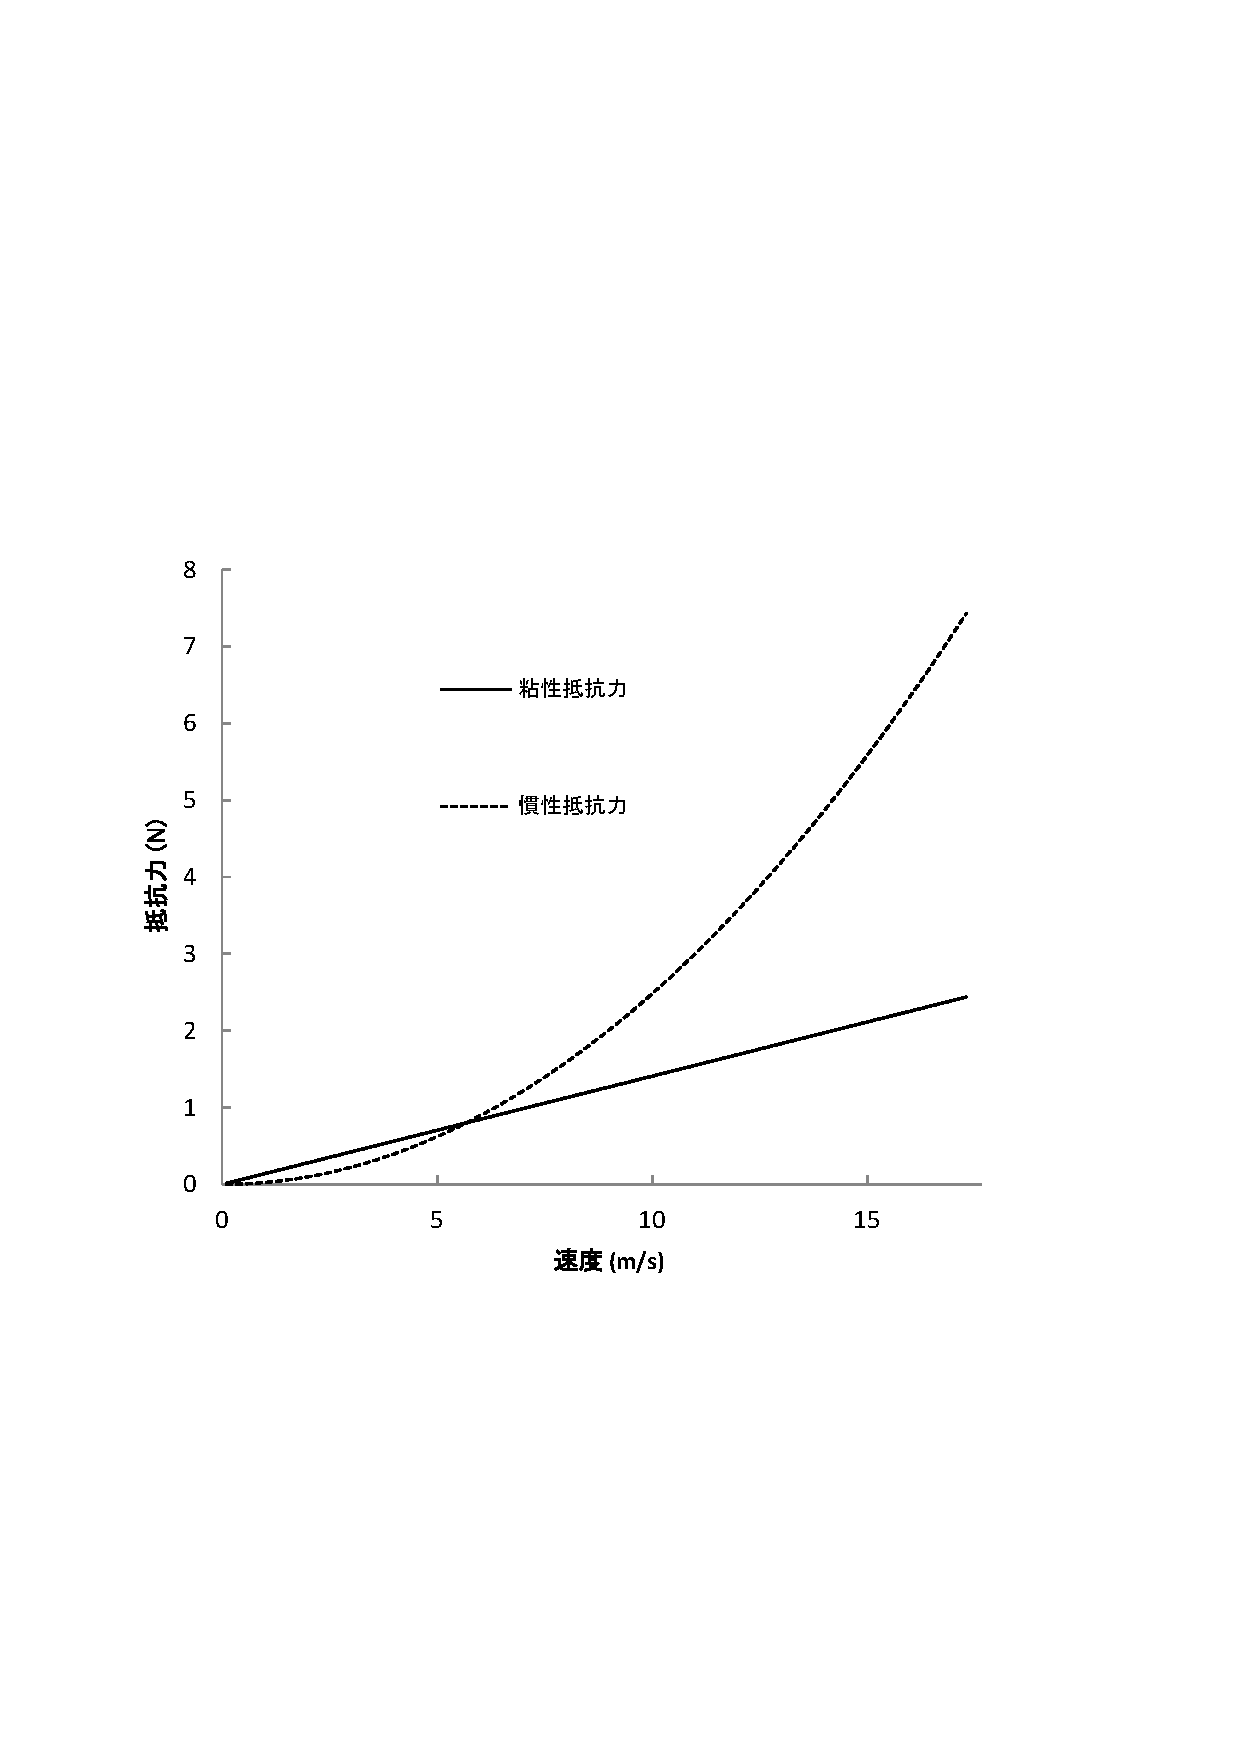
\includegraphics[width=6cm]{s-粘性抵抗と慣性抵抗.pdf}
  \caption{粘性抵抗と慣性抵抗}
  \label{fig.抵抗}
\end{wrapfigure}
 図\ref{fig.抵抗}は,粘性抵抗力$f_v$と慣性抵抗力$f_I$のグラフである~\cite{藤原}.ただし,流体は20℃のグリセリン($\eta=1.495,\rho _0=1.264×10^3$),移動する粒子は半径5mmである.これは力学的にわかりやすい系で描いたグラフであるが,溶液中の高分子のようなミクロな系でも事情はほとんど同じである.速度が小さいところでは粘性抵抗が慣性抵抗を上回っていることが分かる.このグラフでは速度をm/sで記述しているが,高分子の移動はもっと遅い\footnote{例えば,高分子の大きさが1nm程度,移動の速さが$10^{-7}$m/s程度のオーダーである場合で計算してみると,流体が水のときで二つの抵抗力には$10^{10}$程度のひらきがある.(6.71)については文献[5]も参照のこと.}.つまり,移動が十分に遅い場合,慣性抵抗は無視して粘性抵抗だけ考えてしまってよい.これで(6.71),(6.73)式が導出できた.\\
\\




\subsection{Einsteinの関係式(6.72)を導出し,拡散係数を具体的に求める}
これで,あとはEinsteinの関係式さえ理解できれば拡散係数$D_{\scalebox{0.5}{G}}$を具体的に書き表すことができる.この関係式はこういうものだとして使ってしまっても構わないのだろうが,どうせなのでEinsteinが実際に辿ったであろう手順(を単純にしたもの)にしたがって導出してしまおう~\cite{米沢} ~\cite{アイン}.Einsteinの関係式は,溶液の理論と流体論からいくつか式を借用することで導出することができる.
\subsubsection{溶液の理論から 〜力学的に〜}
まずは溶液論に従ってブラウン粒子に働いている力を記述してみよう.$n$モルの溶質が希薄溶液中にあるとき,
\begin{equation}
pV=nRT
\end{equation}
という浸透圧の式が成り立つ.ブラウン粒子にもこの式が適用できる.体積$V$中の
粒子の数密度$\omega$を
\begin{equation}
\omega =\frac{nN_A}{V}
\end{equation}
とすれば,(13)式は
\begin{equation}
p=\frac{RT}{N_A} d=k_B T \omega
\end{equation}
となる.粒子一つあたりに$f$という外力が$x$方向にはたらいているとすると,それは粒子にかかる浸透圧$p$の勾配とつりあうはずである\footnote{少し直感的にはわかりにくい?実際には,Einsteinは熱力学的平衡であることを考えて,エネルギーの極値条件から同じ式を導出している.文献[6] p.223参照.}.
\begin{equation}
\frac{\partial p}{\partial x}=\omega f
\end{equation}
よって
\begin{equation}
f=\frac{1}{d} \frac{\partial}{\partial x} (k_B T \omega)=\frac{1}{d} k_B T \frac{\partial \omega}{\partial x}
\end{equation}
となる.浸透圧による力と外力(外場)がつりあうとして外力を表したわけである.
\subsubsection{流体論から 〜ダイナミカルに〜}
次に,溶液における平衡状態というものを考えてみよう.溶液中で粒子が平衡状態になっているとはどういうことだろうか.これは,「\ding{172}外場$f$のもとでの粒子の運動」と「\ding{173}濃度勾配による拡散の過程」の二つの重ね合わせの結果とみることができる.

先ほどのストークスの法則(12)式によれば,外力$f_{\scalebox{0.5}{V}}$によって粒子に速度
\begin{equation}
v=\frac{f_V}{6 \pi \eta r}
\end{equation}
が生じていると考えられる.つまり,$f_{\scalebox{0.5}{V}}$によって単位時間あたり単位断面積を通って$\omega v$の粒子が通過することになる.これが\ding{172}である.

フィックの第一法則によれば,拡散の起こる方向に,単位面積を通って単位時間に拡散する粒子の個数$J$は,その場所での個数密度の勾配に比例し,
\begin{equation}
J=-D\frac{\partial \omega}{\partial x}
\end{equation}
で表される.これが\ding{173}である.この定数$D$は同じ系を考えているときは,(10)式で出てきた拡散定数と同じなので$D_{\scalebox{0.5}{G}}$としてしまえばよい\footnote{拡散方程式(10)はフィックの第二法則とも呼ばれる.wikipediaでもチラ見してもらえばよいと思う.}.平衡が成り立っているのであれば,単位体積中の粒子の出入りが実質ゼロであり,
\begin{equation}
\omega v+J=0
\end{equation}
すなわち,
\begin{equation}
\frac{\omega f_{\scalebox{0.5}{V}}}{6\pi \eta r}-D_G\frac{\partial \omega}{\partial x}=0
\end{equation}
となる.これで\ding{172}と\ding{173}から平衡の様子を記述できたと同時に,流体論から外力$f_{\scalebox{0.5}{V}}$を表すことができた.

以上で,溶液論と流体論の二つの側面から粒子に働いている力を書くことができた.これらは見方が違うだけで同じものであるはずだ.(17)式と(21)式から二つの力が等しいとして変形すれば,
\begin{equation}
D_G=\frac{k_B T}{6\pi \eta r}=\frac{k_B T}{\zeta}
\end{equation}
Einsteinの関係式を求めることができた.わぁい.これでやっと拡散係数を具体的に書くことができる.半径$r$にはお馴染みの慣性半径を使ってやろう.
\begin{equation}
D_G=\frac{k_B T}{6\pi \eta R_G}
\end{equation}
温度が上がれば動きやすくなり,流体の粘度や高分子のサイズが大きくなれば動きにくくなる.イメージによく合う式である.分子量との関係を知りたければ,(6.57)式
\begin{equation}
R_G \approx N^\nu a
\end{equation}
を使うことにより,
\begin{equation}
D_G \propto M^{- \nu}
\end{equation}
を得る\footnote{教科書ではKirkwoodの近似式なるものが登場して,それを使えばより正確に拡散定数を求めることができると言っている.この式に関する説明は諦めますごめんなさい.興味のある方は文献[10],[11]を.}.$\nu$は理論的には良溶媒で0.6,$\Theta$ 溶媒で0.5らしい.分子量が大きくなれば動きにくくなる.これもイメージによく合う.並進運動終わり.

\section{回転運動}
\subsection{時間相関関数}
次に高分子全体の回転運動を考える.教科書ではまず球体粒子の回転運動を考えている.教科書の図6.13(a)のような中心からの単位ベクトルの動きを追うために,その内積である$\mathrm{cos}\theta (t)$なるものを考えている.というよりも,ランダムな物理量の変動を知りたいときは,冒頭でも述べたように時間相関関数というものを考えることが多い.時間相関関数とは,ここでは
\begin{equation}
C(t)=\langle \bm{u}(t)\cdot \bm{u}(0)\rangle
\end{equation}
という形で書かれているが,一般的に,異なる時刻における確率的な量の積を平均したものである.このように時刻$t=0$と$t=t$で考えれば,観測を開始してからある時間後の変動の具合を知ることができる.

\begin{wrapfigure}{l}{22zw}
  \vspace*{-\intextsep}
  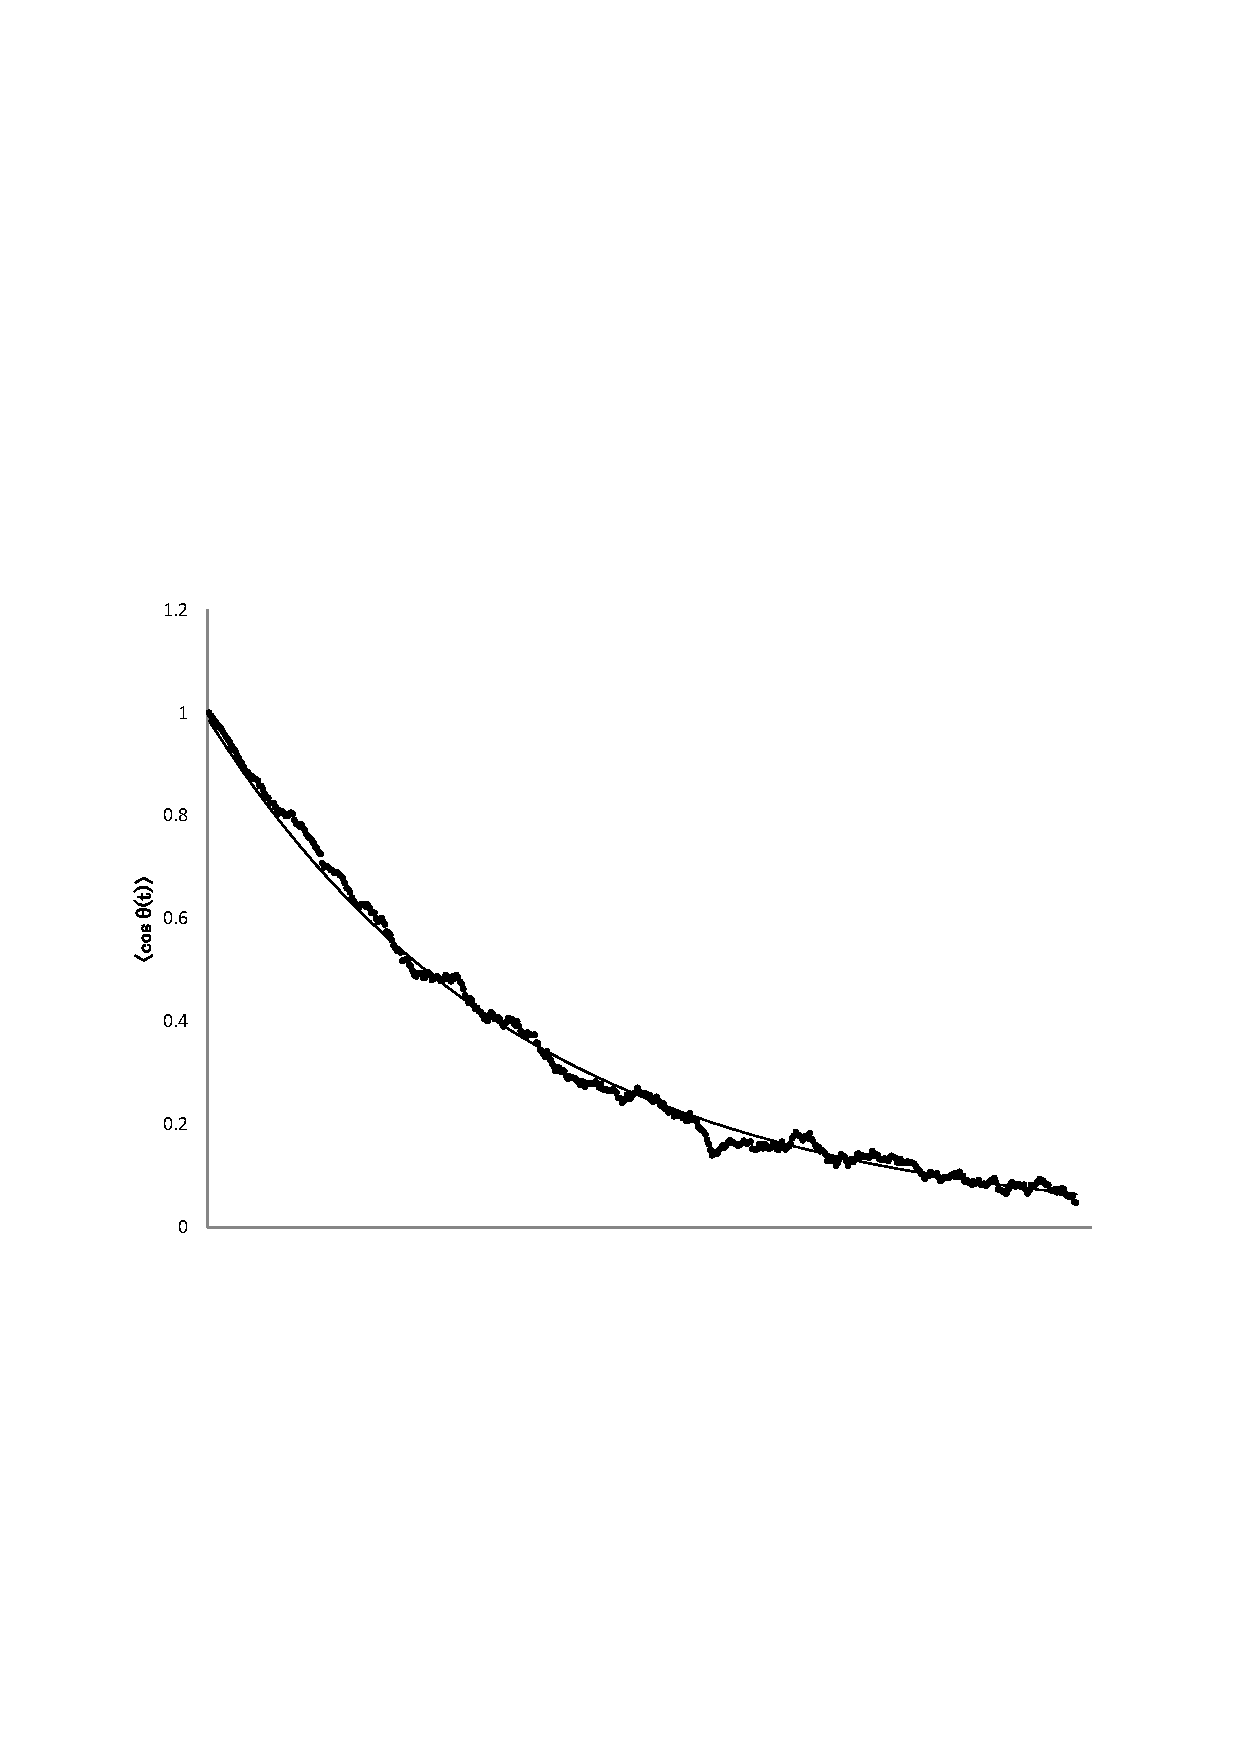
\includegraphics[width=6cm,height=3.5cm]{s-cosの平均.pdf}
  \caption{$\mathrm{cos}\theta (t)$の平均}
  \label{fig.cosの平均}
\end{wrapfigure}
図6.13(b)は球がランダムに回転したときの$\mathrm{cos}\theta (t)$の動きを表したものであり,(c)はその平均である.教科書では「たくさんのデータの平均」と言っている.これは,(b)のようなグラフをたくさんつくり,それらの平均をとるということを示唆しているのだと思う.実際にExcelなどで$\mathrm{cos}\theta (t)$をランダムに動かしたデータをたくさんつくり,それらの平均をとると,(c)に似たグラフが得られる.左の図\ref{fig.cosの平均}はExcel作ってみたグラフである.曲線は指数近似曲線である.

直感的には教科書で述べられている通り,このように多数のデータの平均を取ることをイメージすればよいと思うが,時間相関関数とはこのような考え方とは少し違う気がする.多数のランダムなデータの平均だと考えると,毎回グラフの形が変わってしまう.しかし実際は(6.80)式
\begin{equation}
C(t)=\mathrm{exp}(-t/\tau _r)
\end{equation}
のように,時間相関関数は一つの指数関数に決まる.このことは,次節で説明する線形Langevin方程式というものを考えることで示される.時間相関関数はしばしば「記憶」の指標だと言われる.つまり,$t$だけ時間が経過したときに,その物理量がどれだけ$t$だけ前の自分を覚えているかということを表している.時間相関関数=「記憶の減衰のしかた」と考えるとよいと思う.

\subsection{線形Langevin方程式}
線形Langevin方程式とは,
\begin{equation}
\dot{X}(t)=-\gamma X(t)+R(t)
\end{equation}
という微分方程式のことを指す~\cite{藤坂}~\cite{吉森}.$X(t)$はランダムに変動する量である.この方程式はブラウン運動を記述するために提案された式であり,$X(t)$はブラウン粒子の速度(もしくは運動量),$R(t)$は媒体分子から受けるランダムな力,$-\gamma X(t)$は粒子が動くときに受ける抵抗力に相当する.$\langle X(0)R(t) \rangle$は中身が全くランダムだと考えてゼロと仮定し,両辺に$X(0)$をかけて平均すると,$t\le 0$のとき
\begin{equation}
\langle \dot{X}(t)X(0) \rangle=-\gamma \langle X(t)X(0) \rangle
\end{equation}
$\phi (t)=\langle X(t)X(0) \rangle$とすると,
\begin{equation}
\dot{\phi}(t)=-\gamma \phi(t)
\end{equation}
これを解くと,
\begin{equation}
\phi (t)=\phi(0)e^{-\gamma t}
\end{equation}
となる.$\phi(0)=\langle X^2 (0)\rangle$であるから,
\begin{equation}
\phi (t)=\langle X^2 (0)\rangle e^{-\gamma t}
\end{equation}
$X(t)$が線形Langevin方程式に従うとき,時間相関関数は指数関数になることが示された.今考えている回転(ブラウン)運動は線形Langevin方程式に従う(式(34))ので(6.80)式のように書けるのである.

\subsection{回転緩和時間}
さて,ベクトル$\bm{u}(t)$は長さ1と取っているので,上でいう$\langle X^2 (0)\rangle$は1となる.となると,あと気になるのは回転緩和時間$\tau _r$(上でいう$\gamma$)である\footnote{教科書では回転緩和時間をほぼ$90^\circ$回る時間としているが,実際計算してみるとわかる通り約$68^\circ$回る時間である.}.並進運動では運動の速さの指標として拡散係数を使ったが,今回は緩和時間を使っている.別に回転運動でも拡散係数を使っても構わないと思う.この$\tau _r$を真面目に求めようとするのは,本当にもうどうしようもなくめんどうな仕事である.(6.81)式
\begin{equation}
\tau _r =\frac{4\pi \eta r^3}{k_B T}
\end{equation}
はDebye-Stokes-Einsteinの関係式として知られており,こういうものだとしてしまっても構わないと思う.それでも気になる方は,以下に菊地なりに理解した道のりを示したので文献を集めて辿ってください.

\begin{quote}
\small 
まず,上の$\gamma$という都合上使っただけの定数をわかるもので書き換えなければならない.そのためには文献[8]に従って,粒子が回転する様子を表した時間発展方程式というものを解く必要がある.頑張って解くことができれば,時間相関関数が
\begin{equation}
\langle \bm{u}(t)\cdot \bm{u}(0)\rangle=e^{-2D_r t}
\end{equation}
となることが分かる.ここで$D_r$とは回転の拡散係数と呼ばれるもので,
\begin{equation}
D_r =\frac{k_B T}{\zeta _r}
\end{equation}
というEinsteinの関係式を回転の場合について書いたものに従う.$\zeta _r$も並進運動で出てきた$\zeta$と似たようなもので,回転の摩擦係数と呼ばれるものである.つまり,流体の中で回転する球状物体が受ける摩擦を表す量である.これは,球の半径を$r$,流体の粘度を$\eta$として,
\begin{equation}
\zeta _r =8\pi \eta r^3
\end{equation}
で与えられる.これも有名な式らしい.これがなぜこうなるかは,文献[14]か[15]に従って計算するとわかるかもしれない.文献[10]に従って,トルクと粘性抵抗力が釣り合うと考えて計算しても良いような気がするが,なぜかうまくいかなかった.ここまでの結果を組み合わせると,目標の式が得られる.
\end{quote}
並進運動では半径の1乗が運動の速さに効いていたが,回転運動では半径の3乗で効いている.(6.81)式を見るとわかるように,体積が重要になってくるということだろう.教科書ではこの後,屈曲性高分子の回転について考えている.ただ,やっていることは同じだし,結果も似たようなものなのでここでは詳しくやらない.次節の内部運動と比較するために回転緩和時間の分子量依存性が,
\begin{equation}
\tau _r \propto M^{3\nu}
\end{equation}
となることだけ示しておく.

\section{内部運動}
\subsection{Rouseモデル}
さて,ここまでは並進運動と回転運動という,高分子にしてみれば比較的大きなスケールの運動を見てきた.最後に,それよりも小さいスケールで起きる高分子の内部の運動を考えていこう.内部運動を考えるには,教科書の図6.14にあるようなスプリング‐ビーズモデルというものを考えるとよいらしい.各セグメントをばねがつなぐと考えると,ばねに蓄えられたエネルギーの合計は
\begin{equation}
U=\frac{1}{2}k \sum_{i=2} ^{N}(\bf{R}_\mathit{i} -\bf{R}_\mathit{i-1})^\mathrm{2}
\end{equation}
である.このモデルにおいて運動方程式を立てると,
\begin{equation}
\frac{\mathit{d}\bf{R}_ \mathit{i}}{\mathit{d}t}=\frac{1}{\zeta}(-\frac{\partial U}{\partial \bf{R}_\mathit{i}}+\bf{f}_\mathit{i}) = \mathit{\frac{\mathrm{3}k_B T}{\zeta a^\mathrm{2}}}(\bf{R}_\mathit{i+1}+\bf{R}_\mathit{i-1}-\mathrm{2}\bf{R}_\mathit{i})+\frac{\mathrm{1}}{\zeta}\bf{f}_\mathit{i}
\end{equation}
となる.このような運動のモデルをRouseモデルという.結局は連成振動のようなものを考えればよい.つまり,基準座標を導入して運動を分解すればよい.文献[7]では,実際にこの計算を行って,(6.90),(6.91)式を求めている.重要なのは,Rouseモデルでは排除体積効果と流体力学的相互作用を無視していることである.そのため,拡散係数および回転緩和時間の分子量依存性が(6.90),(6.91)式のように
\begin{equation}
D_G \propto M^{-1}
\end{equation}
\begin{equation}
\tau _r \propto M^2
\end{equation}
と,(25),(37)式で求めた結果と異なってしまう.

\subsection{Zimmモデル}
実際の様子を表すために,流体力学的相互作用を組み込んだモデルとしてZimmモデルというものが提唱されている.やはり文献[7]に詳しい計算が載っているが,Zimmモデルで計算すると,
\begin{equation}
D_G \propto M^{1/2}
\end{equation}
\begin{equation}
\tau _r \propto M^{3/2}
\end{equation}
となり,これまでに求めた分子量依存性とよく一致する.また,Zimmモデルには排除体積効果も組み込むことができる.排除体積効果を加味すると,(6.74),(6.81)式のような半径依存性
\begin{equation}
D_G \propto r^{-1}
\end{equation}
\begin{equation}
\tau _r \propto r^3
\end{equation}
も示される.


\begin{thebibliography}{99}
\bibitem{米沢}
 米沢富美子(1986) 『ブラウン運動』 共立出版
\bibitem{戸田}
 戸田盛和,久保亮五(1972) 『統計物理学』 岩波書店
\bibitem{小岩}
 小岩昌宏,中嶋英雄(2009) 『材料における拡散』 内田老鶴圃
\bibitem{巽}
 巽友正(1982) 『流体力学』 培風館
\bibitem{林}
 林茂雄(2007) 『移動現象論入門』 東洋書店
\bibitem{アイン}
 湯川秀樹他(1971) 『アインシュタイン選集1』 共立出版
\bibitem{野瀬}
 野瀬卓平他(1997) 『大学院 高分子科学』 講談社サイエンティフィク
\bibitem{土井}
 土井正男(2010) 『ソフトマター物理学入門』 岩波書店
\bibitem{藤原}
 藤原邦男(1984) 『物理学序論としての力学』 東京大学出版会
\bibitem{Doi}
 M. Doi and S. F. Edwards {\it The Theory of Polymer Dynamics}; Oxford, 1986; p106
\bibitem{Kirkwood}
 Kirkwood, J. G., {\it J. Polym. Sci.} {\bf 12} , 1 (1954)
\bibitem{藤坂}
 藤坂博一(1998) 『非平衡系の統計力学』 産業図書
\bibitem{吉森}
 九州大学 吉森明 2007年度 非平衡物理学講義ノート6

 http://www.cmt.phys.kyushu-u.ac.jp/~A.Yoshimori/
\bibitem{Perez}
 A. Perez-Madrid and J. M. Rubi {\it Physica}{\bf 132A}(1985) 438.
\bibitem{伊東}
 東京工業大学化学工学専攻 伊東研究室 ホームページ 「流体中の粒子・気泡の運動」

 http://chemeng.in.coocan.jp/fl/fl08a.html
\end{thebibliography}



\end{document}
